% !TeX program = xelatex
\documentclass[12pt, a4paper]{article}
\usepackage{amsmath}
\usepackage{xeCJK}
\usepackage{amsmath}
\usepackage{amssymb}
\usepackage{xcolor}
\usepackage{parskip}
\usepackage{tikz}
\usepackage{enumitem}
\usepackage[most]{tcolorbox}

\newenvironment{definitionbox}
  {\begin{tcolorbox}[colback=white, colframe=black, boxrule=0.8pt, arc=0pt, left=2pt, right=2pt, top=2pt, bottom=2pt]
  \textbf{【Definition】}}
  {\end{tcolorbox}}

\setmainfont{Latin Modern Roman}
\setCJKmainfont{Noto Serif CJK TC}

\title{Ch7. Sampling}
\begin{document}
\section*{Impulse-Train Sampling}
將 $x(t)$ 用 $p(t)$ 以 $T$ 週期進行採樣
\begin{align*}
	p(t) &= \sum_{n = -\infty}^{\infty} \delta(t -nT) \\
	x_p(t) &= x(t)p(t)
\end{align*}


\subsection*{Example}
\begin{center}
\tikzset{every picture/.style={line width=0.75pt}} %set default line width to 0.75pt        

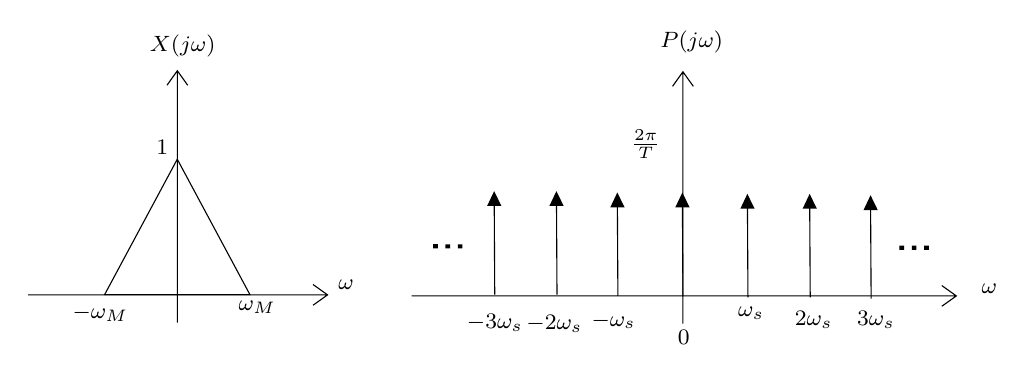
\begin{tikzpicture}[x=0.75pt,y=0.75pt,yscale=-1,xscale=1]
%uncomment if require: \path (0,300); %set diagram left start at 0, and has height of 300

%Shape: Axis 2D [id:dp2501717951491259] 
\draw  (128.17,187.41) -- (272.38,187.41)(200.01,79.43) -- (200.01,200.8) (265.38,182.41) -- (272.38,187.41) -- (265.38,192.41) (195.01,86.43) -- (200.01,79.43) -- (205.01,86.43)  ;
%Flowchart: Extract [id:dp09645599540268068] 
\draw   (199.98,122.05) -- (234.98,187.28) -- (164.98,187.28) -- cycle ;
%Shape: Axis 2D [id:dp31560896470706823] 
\draw  (312.83,187.91) -- (575.32,187.91)(443.6,79.93) -- (443.6,201.3) (568.32,182.91) -- (575.32,187.91) -- (568.32,192.91) (438.6,86.93) -- (443.6,79.93) -- (448.6,86.93)  ;
%Straight Lines [id:da9808693677057245] 
\draw    (443.6,187.91) -- (443.34,141.08) ;
\draw [shift={(443.32,138.08)}, rotate = 89.68] [fill={rgb, 255:red, 0; green, 0; blue, 0 }  ][line width=0.08]  [draw opacity=0] (7.14,-3.43) -- (0,0) -- (7.14,3.43) -- cycle    ;
%Straight Lines [id:da5285540387054449] 
\draw    (474.93,188.58) -- (474.67,141.75) ;
\draw [shift={(474.65,138.75)}, rotate = 89.68] [fill={rgb, 255:red, 0; green, 0; blue, 0 }  ][line width=0.08]  [draw opacity=0] (7.14,-3.43) -- (0,0) -- (7.14,3.43) -- cycle    ;
%Straight Lines [id:da17609034512871435] 
\draw    (504.93,188.58) -- (504.67,141.75) ;
\draw [shift={(504.65,138.75)}, rotate = 89.68] [fill={rgb, 255:red, 0; green, 0; blue, 0 }  ][line width=0.08]  [draw opacity=0] (7.14,-3.43) -- (0,0) -- (7.14,3.43) -- cycle    ;
%Straight Lines [id:da009720405873485993] 
\draw    (534.27,189.24) -- (534,142.41) ;
\draw [shift={(533.99,139.41)}, rotate = 89.68] [fill={rgb, 255:red, 0; green, 0; blue, 0 }  ][line width=0.08]  [draw opacity=0] (7.14,-3.43) -- (0,0) -- (7.14,3.43) -- cycle    ;
%Straight Lines [id:da6840473852554992] 
\draw    (352.93,187.24) -- (352.67,140.41) ;
\draw [shift={(352.65,137.41)}, rotate = 89.68] [fill={rgb, 255:red, 0; green, 0; blue, 0 }  ][line width=0.08]  [draw opacity=0] (7.14,-3.43) -- (0,0) -- (7.14,3.43) -- cycle    ;
%Straight Lines [id:da08954720790348947] 
\draw    (382.93,187.24) -- (382.67,140.41) ;
\draw [shift={(382.65,137.41)}, rotate = 89.68] [fill={rgb, 255:red, 0; green, 0; blue, 0 }  ][line width=0.08]  [draw opacity=0] (7.14,-3.43) -- (0,0) -- (7.14,3.43) -- cycle    ;
%Straight Lines [id:da43583537477910883] 
\draw    (412.27,187.91) -- (412,141.08) ;
\draw [shift={(411.99,138.08)}, rotate = 89.68] [fill={rgb, 255:red, 0; green, 0; blue, 0 }  ][line width=0.08]  [draw opacity=0] (7.14,-3.43) -- (0,0) -- (7.14,3.43) -- cycle    ;
%Straight Lines [id:da299678143895422] 
\draw [line width=1.5]  [dash pattern={on 1.69pt off 2.76pt}]  (547.93,164.67) -- (565.32,164.75) ;
%Straight Lines [id:da2138223536994116] 
\draw [line width=1.5]  [dash pattern={on 1.69pt off 2.76pt}]  (323.27,164) -- (340.65,164.08) ;

% Text Node
\draw (188.69,111.51) node [anchor=north west][inner sep=0.75pt]  [font=\footnotesize]  {$1$};
% Text Node
\draw (148.29,190.91) node [anchor=north west][inner sep=0.75pt]  [font=\footnotesize]  {$-\omega _{M}$};
% Text Node
\draw (228.29,188.91) node [anchor=north west][inner sep=0.75pt]  [font=\footnotesize]  {$\omega _{M}$};
% Text Node
\draw (276.29,179.11) node [anchor=north west][inner sep=0.75pt]  [font=\footnotesize]  {$\omega $};
% Text Node
\draw (185.49,61.11) node [anchor=north west][inner sep=0.75pt]  [font=\footnotesize]  {$X( j\omega )$};
% Text Node
\draw (417.36,106.68) node [anchor=north west][inner sep=0.75pt]  [font=\footnotesize]  {$\frac{2\pi }{T}$};
% Text Node
\draw (398.29,194.74) node [anchor=north west][inner sep=0.75pt]  [font=\footnotesize]  {$-\omega _{s}$};
% Text Node
\draw (468.96,192.08) node [anchor=north west][inner sep=0.75pt]  [font=\footnotesize]  {$\omega _{s}$};
% Text Node
\draw (586.29,180.94) node [anchor=north west][inner sep=0.75pt]  [font=\footnotesize]  {$\omega $};
% Text Node
\draw (431.49,58.94) node [anchor=north west][inner sep=0.75pt]  [font=\footnotesize]  {$P( j\omega )$};
% Text Node
\draw (439.93,203.4) node [anchor=north west][inner sep=0.75pt]  [font=\footnotesize]  {$0$};
% Text Node
\draw (496.29,194.08) node [anchor=north west][inner sep=0.75pt]  [font=\footnotesize]  {$2\omega _{s}$};
% Text Node
\draw (526.29,194.08) node [anchor=north west][inner sep=0.75pt]  [font=\footnotesize]  {$3\omega _{s}$};
% Text Node
\draw (366.96,196.08) node [anchor=north west][inner sep=0.75pt]  [font=\footnotesize]  {$-2\omega _{s}$};
% Text Node
\draw (338.29,195.41) node [anchor=north west][inner sep=0.75pt]  [font=\footnotesize]  {$-3\omega _{s}$};


\end{tikzpicture}
\end{center}

若 $x(t)$ 的 Furier transorm 為三角波, 其中 $\omega_s = 2\pi/T$,可得
\begin{align*}
	X_p(j\omega) = \frac{1}{2\pi} \int_{-\infty}^{\infty} X(j\theta)P(j(\omega - \theta)) \\
	P(j \omega) = \frac{2 \pi}{T} \sum_{k=-\infty}^{\infty} \delta(\omega - k \omega_{s}) \\
	X_p(j \omega) = \frac{1}{T} \sum_{k = -\infty}^{\infty} X(j(\omega - k \omega_{s}))
\end{align*}

\textbf{When $\omega_{c} > 2 \omega_{M}$} \\
不會有重複的 X(j($\omega - k\omega_{s}$)

\begin{center}
\tikzset{every picture/.style={line width=0.75pt}} %set default line width to 0.75pt        

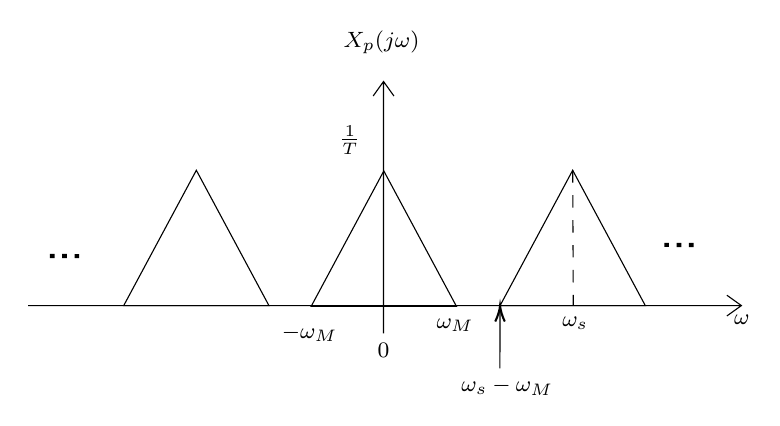
\begin{tikzpicture}[x=0.75pt,y=0.75pt,yscale=-1,xscale=1]
%uncomment if require: \path (0,300); %set diagram left start at 0, and has height of 300

%Shape: Axis 2D [id:dp31560896470706823] 
\draw  (141.83,199.91) -- (485.43,199.91)(313.01,91.93) -- (313.01,213.3) (478.43,194.91) -- (485.43,199.91) -- (478.43,204.91) (308.01,98.93) -- (313.01,91.93) -- (318.01,98.93)  ;
%Straight Lines [id:da299678143895422] 
\draw [line width=1.5]  [dash pattern={on 1.69pt off 2.76pt}]  (448.27,170.67) -- (465.65,170.75) ;
%Straight Lines [id:da2138223536994116] 
\draw [line width=1.5]  [dash pattern={on 1.69pt off 2.76pt}]  (152.27,176) -- (169.65,176.08) ;
%Flowchart: Extract [id:dp965124752016053] 
\draw   (313.15,135.05) -- (348.15,200.28) -- (278.15,200.28) -- cycle ;
%Flowchart: Extract [id:dp7190091988561138] 
\draw   (404.15,134.72) -- (439.15,199.94) -- (369.15,199.94) -- cycle ;
%Flowchart: Extract [id:dp40019246436643474] 
\draw   (222.82,134.72) -- (257.82,199.94) -- (187.82,199.94) -- cycle ;
%Straight Lines [id:da9334564668608473] 
\draw  [dash pattern={on 4.5pt off 4.5pt}]  (404.15,134.72) -- (404.44,199.71) ;
%Straight Lines [id:da4351686642014716] 
\draw    (369.08,230.1) -- (369.15,201.94) ;
\draw [shift={(369.15,199.94)}, rotate = 90.12] [color={rgb, 255:red, 0; green, 0; blue, 0 }  ][line width=0.75]    (7.65,-2.3) .. controls (4.86,-0.97) and (2.31,-0.21) .. (0,0) .. controls (2.31,0.21) and (4.86,0.98) .. (7.65,2.3)   ;

% Text Node
\draw (337.29,204.91) node [anchor=north west][inner sep=0.75pt]  [font=\footnotesize]  {$\omega _{M}$};
% Text Node
\draw (290.36,112.01) node [anchor=north west][inner sep=0.75pt]  [font=\footnotesize]  {$\frac{1}{T}$};
% Text Node
\draw (349.29,233.74) node [anchor=north west][inner sep=0.75pt]  [font=\footnotesize]  {$\omega _{s} -\omega _{M}$};
% Text Node
\draw (397.86,204.36) node [anchor=north west][inner sep=0.75pt]  [font=\footnotesize]  {$\omega _{s}$};
% Text Node
\draw (480.62,202.94) node [anchor=north west][inner sep=0.75pt]  [font=\footnotesize]  {$\omega $};
% Text Node
\draw (292.49,66.28) node [anchor=north west][inner sep=0.75pt]  [font=\footnotesize]  {$X_{p}( j\omega )$};
% Text Node
\draw (308.93,216.73) node [anchor=north west][inner sep=0.75pt]  [font=\footnotesize]  {$0$};
% Text Node
\draw (262.79,207.91) node [anchor=north west][inner sep=0.75pt]  [font=\footnotesize]  {$-\omega _{M}$};
\end{tikzpicture}
\end{center}
	
\textbf{When $\omega_{s} < k \omega_{M}$} \\
$X(j(\omega - k \omega_{s}))$ 會有重疊,訊號失真無法還原

\begin{center}
		

\tikzset{every picture/.style={line width=0.75pt}} %set default line width to 0.75pt        

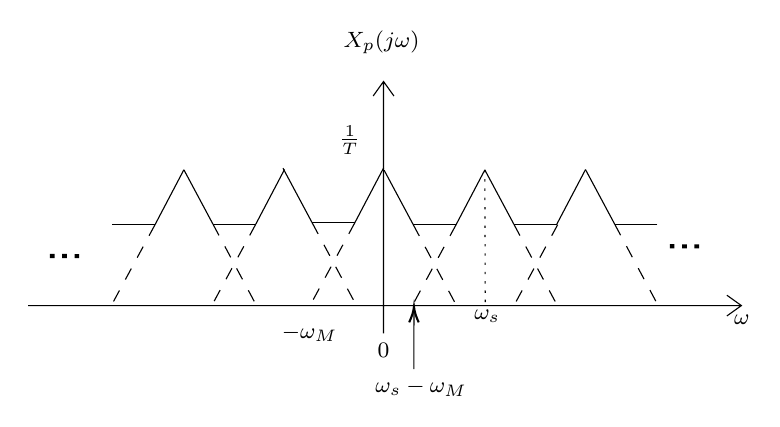
\begin{tikzpicture}[x=0.75pt,y=0.75pt,yscale=-1,xscale=1]
%uncomment if require: \path (0,300); %set diagram left start at 0, and has height of 300

%Shape: Axis 2D [id:dp31560896470706823] 
\draw  (141.83,199.91) -- (485.43,199.91)(313.01,91.93) -- (313.01,213.3) (478.43,194.91) -- (485.43,199.91) -- (478.43,204.91) (308.01,98.93) -- (313.01,91.93) -- (318.01,98.93)  ;
%Straight Lines [id:da299678143895422] 
\draw [line width=1.5]  [dash pattern={on 1.69pt off 2.76pt}]  (450.93,171.33) -- (468.32,171.41) ;
%Straight Lines [id:da2138223536994116] 
\draw [line width=1.5]  [dash pattern={on 1.69pt off 2.76pt}]  (152.27,176) -- (169.65,176.08) ;
%Straight Lines [id:da4351686642014716] 
\draw    (327.62,230.5) -- (327.68,202.34) ;
\draw [shift={(327.68,200.34)}, rotate = 90.12] [color={rgb, 255:red, 0; green, 0; blue, 0 }  ][line width=0.75]    (7.65,-2.3) .. controls (4.86,-0.97) and (2.31,-0.21) .. (0,0) .. controls (2.31,0.21) and (4.86,0.98) .. (7.65,2.3)   ;
%Straight Lines [id:da2964145013306032] 
\draw    (327.4,161.05) -- (313.32,134.72) ;
%Straight Lines [id:da5104837904613073] 
\draw    (347.9,161.05) -- (327.4,161.05) ;
%Straight Lines [id:da3430805168085034] 
\draw    (361.82,134.55) -- (347.9,161.05) ;
%Straight Lines [id:da04518429929755652] 
\draw    (278.65,160.05) -- (264.57,133.72) ;
%Straight Lines [id:da1695795690976064] 
\draw    (299.15,160.05) -- (278.65,160.05) ;
%Straight Lines [id:da6160247115520963] 
\draw    (313.07,133.55) -- (299.15,160.05) ;
%Straight Lines [id:da42858143685852323] 
\draw    (230.9,160.8) -- (216.82,134.47) ;
%Straight Lines [id:da034831085387855065] 
\draw    (251.4,160.8) -- (230.9,160.8) ;
%Straight Lines [id:da8725713894560059] 
\draw    (265.32,134.3) -- (251.4,160.8) ;
%Straight Lines [id:da617646655290906] 
\draw    (375.9,160.88) -- (361.82,134.55) ;
%Straight Lines [id:da6728525056626149] 
\draw    (396.4,160.88) -- (375.9,160.88) ;
%Straight Lines [id:da23453371562654612] 
\draw    (410.32,134.39) -- (396.4,160.88) ;
%Straight Lines [id:da5843066775342645] 
\draw    (424.4,160.71) -- (410.32,134.39) ;
%Straight Lines [id:da7865883590928362] 
\draw  [dash pattern={on 4.5pt off 4.5pt}]  (251.4,160.8) -- (230.32,199.78) ;
%Straight Lines [id:da7610783936373235] 
\draw  [dash pattern={on 4.5pt off 4.5pt}]  (230.9,160.8) -- (251.82,199.94) ;
%Straight Lines [id:da3922323317403086] 
\draw  [dash pattern={on 4.5pt off 4.5pt}]  (278.65,160.05) -- (299.57,199.19) ;
%Straight Lines [id:da4123706752801116] 
\draw  [dash pattern={on 4.5pt off 4.5pt}]  (299.15,160.05) -- (278.07,199.03) ;
%Straight Lines [id:da7943252887276127] 
\draw  [dash pattern={on 4.5pt off 4.5pt}]  (327.4,161.05) -- (348.32,200.19) ;
%Straight Lines [id:da02939616488595098] 
\draw  [dash pattern={on 4.5pt off 4.5pt}]  (347.9,161.05) -- (326.82,200.03) ;
%Straight Lines [id:da0013254956968209441] 
\draw  [dash pattern={on 4.5pt off 4.5pt}]  (375.9,160.88) -- (396.82,200.03) ;
%Straight Lines [id:da15178878667017526] 
\draw  [dash pattern={on 4.5pt off 4.5pt}]  (396.9,160.96) -- (375.82,199.94) ;
%Straight Lines [id:da14959078033826245] 
\draw    (202.9,160.96) -- (182.4,160.96) ;
%Straight Lines [id:da009401093638852998] 
\draw    (216.82,134.47) -- (202.9,160.96) ;
%Straight Lines [id:da6476558213050856] 
\draw  [dash pattern={on 4.5pt off 4.5pt}]  (202.9,160.96) -- (181.82,199.94) ;
%Straight Lines [id:da5779633184373707] 
\draw    (444.9,160.71) -- (424.4,160.71) ;
%Straight Lines [id:da18480648008088862] 
\draw  [dash pattern={on 4.5pt off 4.5pt}]  (424.4,160.71) -- (445.32,199.86) ;
%Straight Lines [id:da524631471954088] 
\draw  [dash pattern={on 0.84pt off 2.51pt}]  (361.82,134.55) -- (362.01,198.87) ;

% Text Node
\draw (290.36,112.01) node [anchor=north west][inner sep=0.75pt]  [font=\footnotesize]  {$\frac{1}{T}$};
% Text Node
\draw (307.82,234.14) node [anchor=north west][inner sep=0.75pt]  [font=\footnotesize]  {$\omega _{s} -\omega _{M}$};
% Text Node
\draw (355.46,200.76) node [anchor=north west][inner sep=0.75pt]  [font=\footnotesize]  {$\omega _{s}$};
% Text Node
\draw (480.62,202.94) node [anchor=north west][inner sep=0.75pt]  [font=\footnotesize]  {$\omega $};
% Text Node
\draw (292.49,66.28) node [anchor=north west][inner sep=0.75pt]  [font=\footnotesize]  {$X_{p}( j\omega )$};
% Text Node
\draw (308.93,216.73) node [anchor=north west][inner sep=0.75pt]  [font=\footnotesize]  {$0$};
% Text Node
\draw (262.79,207.91) node [anchor=north west][inner sep=0.75pt]  [font=\footnotesize]  {$-\omega _{M}$};
\end{tikzpicture}
\end{center}

\section*{Sample Theorem}
\begin{definitionbox}
	\begin{enumerate}[label=\arabic*.]
		\item $x(t)$ be a band-limited signal
		\item $X(j \omega) = 0$ for $\left| \omega \right| > \omega_{M}$
		\item $x_p(t)$ 復原成原本的 $x(t)$ 條件為 $\omega_{s} > 2 \omega_{M}$
	\end{enumerate}
\end{definitionbox}

\section*{Reconstruction}
\subsection*{Interpolation}
常用的 reconstruction 方法,將取樣的點連呈直線,只要取樣法滿足 $\omega_{s} > 2 \omega_{M}$,直線段連接會和原本連續訊號相似。否則當 $\omega_{s} \ngtr 2 \omega_{M}$ 會 aliasing。

\begin{center}
	

\tikzset{every picture/.style={line width=0.75pt}} %set default line width to 0.75pt        

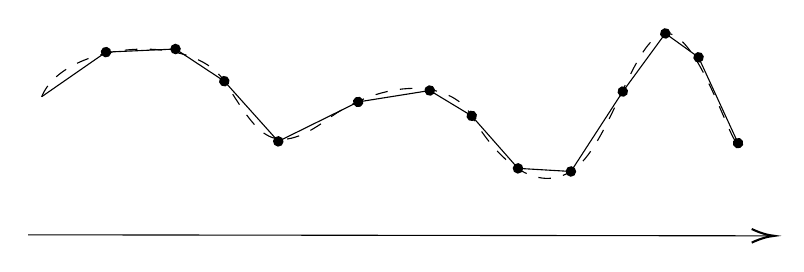
\begin{tikzpicture}[x=0.75pt,y=0.75pt,yscale=-1,xscale=1]
%uncomment if require: \path (0,300); %set diagram left start at 0, and has height of 300

%Straight Lines [id:da8670765054505492] 
\draw    (88.82,210.31) -- (446.32,210.81) ;
\draw [shift={(448.32,210.81)}, rotate = 180.08] [color={rgb, 255:red, 0; green, 0; blue, 0 }  ][line width=0.75]    (10.93,-3.29) .. controls (6.95,-1.4) and (3.31,-0.3) .. (0,0) .. controls (3.31,0.3) and (6.95,1.4) .. (10.93,3.29)   ;
%Curve Lines [id:da4179697983251872] 
\draw  [dash pattern={on 4.5pt off 4.5pt}]  (95.28,143.79) .. controls (105.78,117.79) and (167.43,111.97) .. (183.28,136.29) .. controls (199.13,160.6) and (205.28,174.79) .. (232.78,154.79) .. controls (260.28,134.79) and (292.28,135.29) .. (302.49,153.01) .. controls (312.7,170.72) and (331.28,191.29) .. (350.28,179.79) .. controls (369.28,168.29) and (380.11,114.76) .. (395.78,113.29) .. controls (411.44,111.81) and (427.69,168.49) .. (430.82,166.14) ;
%Straight Lines [id:da904744114779353] 
\draw    (95.28,143.79) -- (126.28,122.29) ;
\draw [shift={(126.28,122.29)}, rotate = 325.26] [color={rgb, 255:red, 0; green, 0; blue, 0 }  ][fill={rgb, 255:red, 0; green, 0; blue, 0 }  ][line width=0.75]      (0, 0) circle [x radius= 2.01, y radius= 2.01]   ;
%Straight Lines [id:da8500065692422741] 
\draw    (126.28,122.29) -- (159.78,120.79) ;
\draw [shift={(159.78,120.79)}, rotate = 357.44] [color={rgb, 255:red, 0; green, 0; blue, 0 }  ][fill={rgb, 255:red, 0; green, 0; blue, 0 }  ][line width=0.75]      (0, 0) circle [x radius= 2.01, y radius= 2.01]   ;
%Straight Lines [id:da2367173183063146] 
\draw    (159.78,120.79) -- (183.28,136.29) ;
\draw [shift={(183.28,136.29)}, rotate = 33.41] [color={rgb, 255:red, 0; green, 0; blue, 0 }  ][fill={rgb, 255:red, 0; green, 0; blue, 0 }  ][line width=0.75]      (0, 0) circle [x radius= 2.01, y radius= 2.01]   ;
%Straight Lines [id:da06929368105956546] 
\draw    (183.28,136.29) -- (209.28,165.29) ;
\draw [shift={(209.28,165.29)}, rotate = 48.12] [color={rgb, 255:red, 0; green, 0; blue, 0 }  ][fill={rgb, 255:red, 0; green, 0; blue, 0 }  ][line width=0.75]      (0, 0) circle [x radius= 2.01, y radius= 2.01]   ;
%Straight Lines [id:da7754083498279123] 
\draw    (209.28,165.29) -- (247.78,146.29) ;
\draw [shift={(247.78,146.29)}, rotate = 333.73] [color={rgb, 255:red, 0; green, 0; blue, 0 }  ][fill={rgb, 255:red, 0; green, 0; blue, 0 }  ][line width=0.75]      (0, 0) circle [x radius= 2.01, y radius= 2.01]   ;
%Straight Lines [id:da62323962853928] 
\draw    (247.78,146.29) -- (282.28,140.79) ;
\draw [shift={(282.28,140.79)}, rotate = 350.94] [color={rgb, 255:red, 0; green, 0; blue, 0 }  ][fill={rgb, 255:red, 0; green, 0; blue, 0 }  ][line width=0.75]      (0, 0) circle [x radius= 2.01, y radius= 2.01]   ;
%Straight Lines [id:da040207186110147175] 
\draw    (282.28,140.79) -- (302.49,153.01) ;
\draw [shift={(302.49,153.01)}, rotate = 31.16] [color={rgb, 255:red, 0; green, 0; blue, 0 }  ][fill={rgb, 255:red, 0; green, 0; blue, 0 }  ][line width=0.75]      (0, 0) circle [x radius= 2.01, y radius= 2.01]   ;
%Straight Lines [id:da5541314072441447] 
\draw    (302.49,153.01) -- (324.78,178.29) ;
\draw [shift={(324.78,178.29)}, rotate = 48.6] [color={rgb, 255:red, 0; green, 0; blue, 0 }  ][fill={rgb, 255:red, 0; green, 0; blue, 0 }  ][line width=0.75]      (0, 0) circle [x radius= 2.01, y radius= 2.01]   ;
%Straight Lines [id:da6090812431666875] 
\draw    (324.78,178.29) -- (350.28,179.79) ;
\draw [shift={(350.28,179.79)}, rotate = 3.37] [color={rgb, 255:red, 0; green, 0; blue, 0 }  ][fill={rgb, 255:red, 0; green, 0; blue, 0 }  ][line width=0.75]      (0, 0) circle [x radius= 2.01, y radius= 2.01]   ;
%Straight Lines [id:da21443291439660972] 
\draw    (350.28,179.79) -- (375.28,141.29) ;
\draw [shift={(375.28,141.29)}, rotate = 303] [color={rgb, 255:red, 0; green, 0; blue, 0 }  ][fill={rgb, 255:red, 0; green, 0; blue, 0 }  ][line width=0.75]      (0, 0) circle [x radius= 2.01, y radius= 2.01]   ;
%Straight Lines [id:da12857095014539732] 
\draw    (375.28,141.29) -- (395.78,113.29) ;
\draw [shift={(395.78,113.29)}, rotate = 306.21] [color={rgb, 255:red, 0; green, 0; blue, 0 }  ][fill={rgb, 255:red, 0; green, 0; blue, 0 }  ][line width=0.75]      (0, 0) circle [x radius= 2.01, y radius= 2.01]   ;
%Straight Lines [id:da12017961456238391] 
\draw    (395.78,113.29) -- (411.78,124.79) ;
\draw [shift={(411.78,124.79)}, rotate = 35.71] [color={rgb, 255:red, 0; green, 0; blue, 0 }  ][fill={rgb, 255:red, 0; green, 0; blue, 0 }  ][line width=0.75]      (0, 0) circle [x radius= 2.01, y radius= 2.01]   ;
%Straight Lines [id:da0936256247853624] 
\draw    (411.78,124.79) -- (430.82,166.14) ;
\draw [shift={(430.82,166.14)}, rotate = 65.28] [color={rgb, 255:red, 0; green, 0; blue, 0 }  ][fill={rgb, 255:red, 0; green, 0; blue, 0 }  ][line width=0.75]      (0, 0) circle [x radius= 2.01, y radius= 2.01]   ;
\end{tikzpicture}
\end{center}

\begin{tcolorbox}[colback=white, colframe=black, boxrule=0.8pt, arc=0pt, left=2pt, right=2pt, top=2pt, bottom=2pt]
	\textbf{Shannon-Whittaker Sample Theorem} \\
	If $\omega_{s} > 2 \omega_{0}$
	$$
	x(t) = \sum_{n = -\infty}^{\infty}x(nT) \mathrm{sinc} \left( \frac{t - nT}{T} \right), \quad \mathrm{sinc}(u) = \frac{\sin \pi u}{\pi u}
	$$
\end{tcolorbox}

\end{document}

